\chapter{Approach and Preliminary Design}

\section{Approach}
Soon after receiving this project it was decided that we would break the project up into a series of smaller projects that we would complete in series. This decision was made after we realised that the transformation of the provided go-kart to a fully working autonomous vehicle was a goal that we would be unlikely to achieve in the time allotted.

If we start all of the sub-systems in parallel then it is likely that by the final deadline we would have many incomplete subsystems putting a steep learning curve in front of any continuation of our work.

By dividing the project into a series of modules with simple well documented interfaces between each we will ensure that we leave a single clean interface with which any future team can build upon with minimal repetition of work. The sub-projects we have divided this project into are outlined below
\begin{description}
\item[Drive by wire] This is the conversion of the go-kart from a traditional mechanical system to something that can be controlled by a laptop. 

\item[Sensor interfacing] In this module the sensors the system will use to perceive the kart's state and the world around it are chosen. After selection they will be fixed to the kart and interfaced with the control system. 

\item[High level control of systems] The drive by wire module will provide functions that directly relate to the kart's systems such as the angle of the steering wheel, braking force and accelerator position. This module abstracts away low level control from the behavioural layer. An example of this abstraction is using the brake, accelerator and the Hall Effect velocity sensor to implement a closed loop controller for the kart's speed.  

\item[Simple autonomous behaviour] This stage is the development of an simple to implement program for autonomous control of the kart. For example using radio triangulation or computer vision to track a token so that the go-kart can autonomously follow a person or another vehicle.

\item[Complex autonomous behaviour] This module would see the integration of reactive path finding using distance sensors and absolute positioning using GPS into the autonomous go-kart's system. These will enable it to operate as a fully-fledged autonomous vehicle able to operate without any form of human interaction or control. When completed the go-kart will autonomously navigate to a GPS location safely avoiding obstacles along the way.
\end{description}

\section{Braking System}

The go-kart's brakes will be controlled via a linear actuator. This will be
connected by removing the brake pedal and connecting the actuator directly to
the input of the hydraulic brake systems. It was decided to use the existing
hydraulic system rather than attach a controlled actuator directly to the brake
disk. This was done as it allowed the system to be attached and operated with
minimal modifications to the existing kart. Another reason this decision was
made is that actuators with relatively low force and large travel were much more
readily available and cheaper then those with small movement and high force and
the existing hydraulic system already converted this large movement into the
high force required resulting in a cheaper system. Through rough testing it was
determined that a human could apply approximately 300 N to the brake pedal. The
leverage in the brake pedal was estimated at be roughly a 2 to 1 system. This
meant the ideal actuator had to provide 600 N of force to operate the brakes. To
go from full off to fully on the actuator required 30 mm of travel.

The actuator selected to power the brake was a 24V Warner linear m-track1. Its
specifications deviated from our requirements slightly. The actuator had 100mm
of travel more then three times the required making it longer then necessary.
However space was not an issue so this was not seen as a problem. The actuator
could only produce 450 N of force, it has yet to be seen how fast a deceleration
this will allow however as 600N is the maximum a human could reasonably apply we
are confident 450N will be sufficient. In the unlikely event this force proves
too small in testing the large travel of the actuator means it can instead be
mounted to the brake pedal using the leverage to give the required force. The
actuator moves at 15mm per second under load. This means that from off to full
lock takes 2 seconds. This speed is a lot slower then desired however the brake
pads do not actually touch the brake during the first half of the travel. This
dead zone is there to prevent drivers accidentally applying the brakes and to
accommodate different thickness brake pads as they wear. If the servo is
recalibrated on a regular bases this dead zone can be all but removed allowing
full brake control in a second. The main driving decision in the purchase of the
actuator was price. The actuator was an end of line product that had been
heavily discounted to sell this meant that it only cost \$110 NZD including
shipping to New Zealand from America. An actuator of similar specification could
not be located for less then \$220 in the US or within New Zealand for less then
\$300.

\section{Steering System}

The steering on the go-kart operates on a rack and pinion system. The steering
wheel rotates from lock to lock in 270 degrees. At rest on concrete the wheel
requires 7 Nm to turn, this value represents a worst case scenario with
significantly less force required when the kart is moving or on grass. Initially
a servo was going to be used to drive the steering wheel however servos with the
ability to produce 7Nm of continuous torque at a reasonable speed were found to
be both difficult to locate and prohibitively expensive (\$500+). Instead a
system of a DC motor, gearbox and encoder is to be used. For the motor to be
attached the steering column will be removed and the output of the gearbox
will drive the pinion directly with the motor bolted in the space left by the
removed column. %Not necessarily but it reads well.

The motor system selected for use in the go-kart is the IG52-04 52mm gear motor.
It comes with a 1:353 gearbox and a Hall Effect encoder attached to a second
rear output shaft on the motor. This motor was selected as it combined all the
 required system into one convient system which required no assembly on our part.
 Another major reason for its selection was the large difficulty that was
 encountered in finding any reasonbly priced gearbox that could sustain the
 continous torque requirements of the system. This motor produces 10 Nm of continuous torque
which will allow it to easily turn the wheel. Its gearbox output rotates at 10
RPM allowing it to travel from lock to lock in 4.5 seconds. A concern with using
this motor is that it has the ability when stalled to produce a peak torque of
up to 100 Nm. This high torque has the potential to damage the steering system
or the gearbox which is only rated for peak torques of 30 Nm. Because of this it
must be ensured that the wheel is never driven right up till the end of its
travel to prevent the motor stalling against the end and generating these
forces. The encoder must be calibrated upon each setup of the system. This is
because the encoder only outputs change in rotation and the rack may be in any
position when the system is initialised. Because of this limit switches will be
placed on small plates attached to the rack shaft to indicate when it has
reached the end of its travel. On start up the motor will locate both limit
switches to calibrate its location. These limit switches will also act as kill
switches during operation to prevent the motor reaching the end of its travel.

\section{Controlling the motor and actuator}

Both systems operate on 24V. This was done as the go-kart already had a 24V rail
for driving the main motor. Using the same voltage saves money and simplifies
the design as it precludes the need for converters that would have to be capable
of the 12A peak currents produced by the system. Both systems are controlled
through an H-Bridge interfaced with a SAM7 processor connected to a can bus.
These SAM7s take care of all the low level control required to operate the
drives allowing the main control computer to operate them at a high level with
instructions that corresponds to desired behaviour rather low level drive
operation.

The SAM7 responsible for steering will take the desired wheel angle as an input
from the can bus. It will also track the encoder's output to calculate the
turning angle. Running a PID controller between the setpoint and current value
it will send the PID loops output as a PWM signal to the H-bridge.

The design of the linear actuator is similar. The SAM7 will be passed the
current and desired speeds of the go-kart. From this and the voltage output by
the potentiometer built into the linear actuator the error in the actuator's
location will be found. Again a PID controller will drive a PWM signal to the
H-bridge controlling the actuator.

\section{High-level logic and control}

For high level control it was decided to design a system where the go-kart can
be fully controlled by a laptop using a simple USB interface.  There are a few
reasons behind this decision, the biggest one would have to be the much nicer
programming environment presented on a standard PC.  A large availability of
higher level languages and better libraries for any low level stuff that may be
required means that it will be easier to design and build the control system.

This also makes it much simpler to interface to a set of more complex sensors,
doing any sort of computer vision system on an embedded system would require a
lot more effort to design, build and test than doing the same on a standard PC.

To support this simple USB interface a modular design will be employed, a
general overview of the approach can be seen in Fig. \ref{can-design}.

\begin{figure}
  \centering
  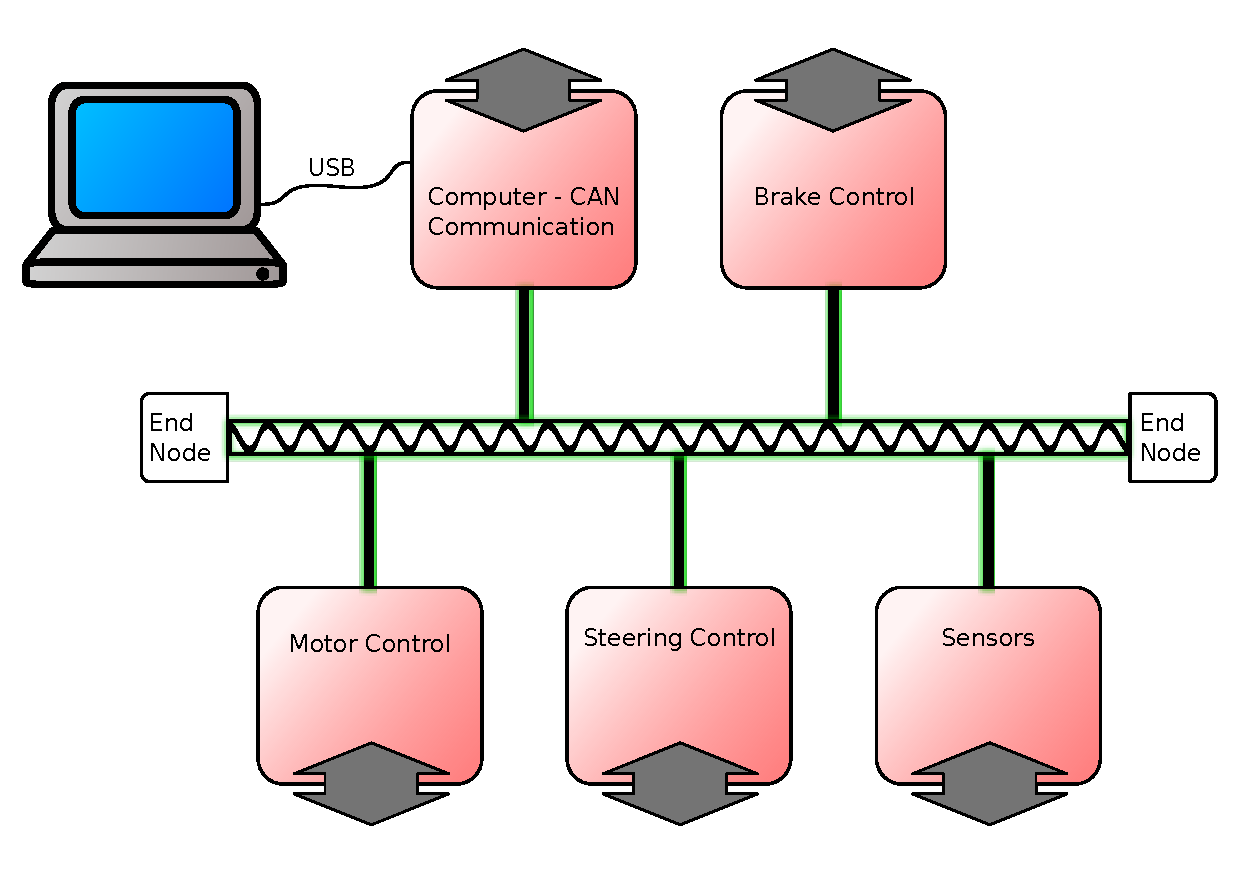
\includegraphics[width=0.8\textwidth]{../../Images/can_diagram.pdf}
  \caption{Basic go-kart control system overview.\label{can-design}}
\end{figure}

\subsection{CAN bus}

The first decision required for the design of the logic boards was what
communication protocol should be used between boards, it would require only a
low data rate but it would have to be able to communicate over at least 3 meters
and be resistant to noise.  Especially because of the PWM controlled DC motor,
the environment could potentially be quite noisy.
% TODO: Last sentence definitely needs re-wording

Our first thoughts on this was the simple serial buses that we had used
previously; Universal Asynchronous Receiver/Transmitter (UART), Serial
Peripheral Interface bus (SPI) and Inter-Integrated Circuit
(I\textsuperscript{2}C).  Unfortunately these buses are limited in range and can
be highly susceptible to noise.

Dr. Michael Hayes (personal correspondence, April 2011) suggested
Controller-Area Network (CAN-bus) or Local Interconnect Network (LIN-bus) as
industry standard bus-systems used in automotive applications.  Because of their
design they are very robust standards that will work well in a high noise
environment.

CAN-bus utilises a high level message-based, multi-master protocol with
automatic priority based arbitration-free transmission.  The original
specification defined up to the transfer layer (link layer in the OSI standard
model), which takes care of tasks such as fault confinement, error detection,
message validation, acknowledgement, arbitration, message framing, transfer rate
and timing and information routing.  The ISO 11898-2 standard defines high-speed
MAC and physical layers to allow a full implementation of the bus.  This
standard utilises a two-wire balanced signalling scheme which allows for high
common noise rejection and is capable of up to 1 Mbit/s transmission rates, far
more than we will be requiring.

LIN-bus is a small, slow network system that is commonly used as a cheap
sub-network of a CAN bus.  It utilises a master-slave architecture without
collision detection and supports up to 16 slaves.  The communications happen
over a single wire capable of up to 19.2 kbit/s with a 40 meter bus.  Again this
would be enough for our limited communications need, and as we only need 5 nodes
the 16 slave limitation doesn't matter.

% TODO: Another paragraph on awesomeness

\subsection{SAM7X}


